\documentclass[a4paper,10pt]{article}
\usepackage[utf8x]{inputenc}
\usepackage[english]{babel}
\usepackage{hyperref}
\usepackage{amsfonts}
\usepackage{graphicx}
\usepackage{amsmath}
\usepackage{subfigure}

\usepackage{placeins}
\usepackage{cleveref}

%opening
\title{TITOLO}
\author{Davide Aversa - Vittorio Perera}

\begin{document}

\maketitle

%\begin{comment}
\begin{abstract}

This report describes the simulation of a quadrotor navigation system based on
ARTag marker recognition and a basic PD controller. The quadrotor can be
controlled with voice commands through an Android application and the Google
speech recognition interface.

The goal of this work is to show the performance and the robustness of this
system. The findings are encouraging and make possible a future implementation
of this work on the real quadrotor.

\end{abstract}
%\end{comment}

\section{Intro}

quadrotor controllato con pd
artag per stima della posiziona
simulazione ROS/Gazebo

\section{Hovering}

\subsection{The hovering problem}

As the first requirement for this project, the quadrotor has to be able to
perform hovering on a single tag. To do this the quadrotor can use only these
data:

\begin{itemize} 
    \item The vector $\hat{x},\hat{y},\hat{z}$ of the estimated position of the
        quadrotor respect to the current active tag\footnote{In the hovering
        problem the active tag corresponds to the only available tag.}.
    \item The vector $\hat{v}_x, \hat{v}_y, \hat{v}_z$ of the estimated
        velocities of the quadrotor. These values are computed by a combination
        of IMU sensor data and an optical flow on the camera input.
\end{itemize}

The quadrotor must use this input to stay in a fixed position respect to the
current active tag. In fact we assume that the desired position is expressed in
the active tag reference frame regardless of the real position in world
coordinates 

This is an important assumption because it greatly simplify the equation
involved and, in addition, it allows to perform target hovering also when we do
not know the real position of the tag in the world frame.

\subsection{Position estimation}

As we said the main sensor input for the quadrotor localization comes from the
ARTag pose estimation from the camera. These values represent an approximation
of the real quadrotor position in a reference frame centered in the active tag.

However the input of ARTag cannot be used directly as reference for the PD
controller of the quadrotor. The ARTag estimation are very noisy an subject to
sensible variations at each frame. To have a more robust estimation we perform a 
low-pass filtering (using an exponential filter) on the ARTag current input
$\hat{\boldsymbol{p}}^{\star}_{t}$.

\begin{equation}
    \hat{\boldsymbol{p}}_{t} = \hat{\boldsymbol{p}}_{t-1} (1-e^{k\Delta{\boldsymbol{p}}}) + \hat{\boldsymbol{p}}^{\star}_{t}(e^{k\Delta{\boldsymbol{p}}})
\end{equation}

where

\begin{equation}
    \Delta{\boldsymbol{p}} = (\hat{\boldsymbol{p}}_{t-1} - \hat{\boldsymbol{p}}_t^\star)^2
\end{equation}

and $k$ is just a real negative constant called \emph{smooth factor}.

funzione PD riferimenti smoothing stima


\section{Navigation}

\subsection{The navigation problem}

Now that our quadrotor knows how to do hovering on a single point, it is time to
add more tags to make possible for it to follow a path.

The quadrotor maintains a list of the existent tags ($S = (s_1,...,s_n)$) and
a pointer (usually an integer index) to the current active tag. At any time we
can order a change for quadrotor active tag and see it moves itself towards the 
selected new active one.

In our simulation we use a simple sequential path: the robot can follow only
one direction: forward or backward. In general it is possible to create more
complex path (for example a tree-like path) with the only limitation that the 
quadrotor camera must see every possible next tag.

\subsection{Tag switch sequence}

The most critical aspect of tag navigation is the \emph{tag switching}
sequence. This sequence is composed by three steps:

\begin{enumerate}
    \item Search for the next tag. Suppose that the quadrotor active tag is
        $s_i$ and the next desired tag is $s_j$. In that case the algorithm
        will search for tag $s_j$ in the camera image still using $s_i$ as
        reference tag.
    \item Switch the active target to $s_j$ updating the desired position
        according to the offset between $s_i$ and $s_j$. This is important
        because switching the active target changes the reference frame of the
        quadrotor and introduces a sensible instant error in the controller
        input. The new desired position is chosen such that position error is
        zero in the switch instant.
    \item Drag the desired position back to its original value.
\end{enumerate}

In our project the point 3 is achieved with a simple linear interpolation:

\begin{equation}
    \boldsymbol{d}(t) = \boldsymbol{d}_f \frac{t-t_0}{T} + (1-\frac{t-t_0}{T})\boldsymbol{d}_i\:\:\: \text{for}\, t_0 \le t \le t_0+T
\end{equation}

where $t_0$ is the instant in which the switching begin, $T$ is the switching
duration, and $\boldsymbol{d}_i$ and $\boldsymbol{d}_f$ is the starting and
final position.


\section{Voice Interface}

After enabling the robot to navigate using ARTags we wanted a simple way to control it and we implemented a Voice Interface. The first step was to find a suitable Automatic Speech Recognizer (ASR); we settled for the Google Speech Recognizer as it currently is one of the best performing over free-form speech and developed and Android application to make use of its API. The goal of this application is to take as input a sound, the spoken commands, and returns a set of possible interpretations to the computer controlling the robot. Figure \ref{fig:tablet_speak} shows the main interface of the application. 

\begin{figure}[h!]
  \centering
    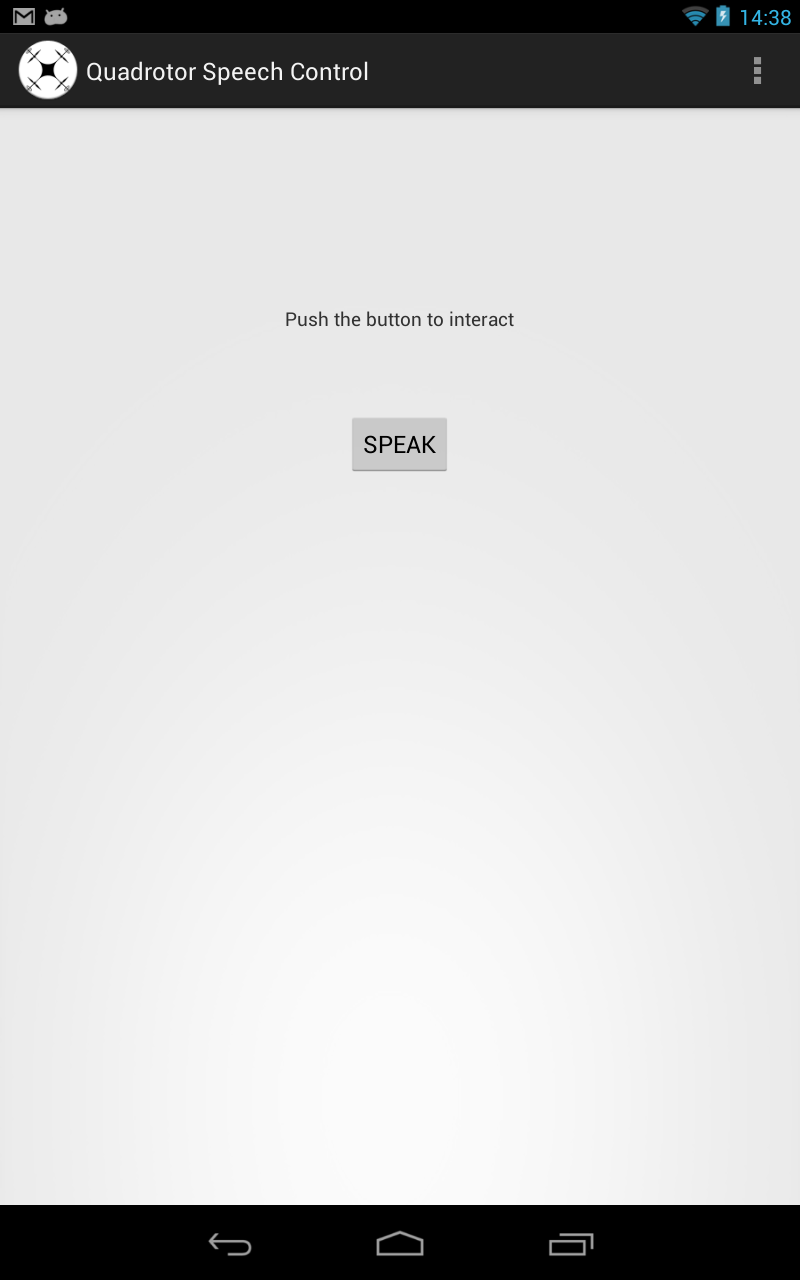
\includegraphics[scale=0.25]{figs/tablet1.png}
  \caption{Main screen from the Android app}
  \label{fig:tablet_speak}
\end{figure}


When using speech to control a robot a wide set of problem arise; first of all people expect from robots to do much more then what they are currently able to, moreover they use many different ways to express the same command and, last, speech recognition technologies often introduce errors in the transcription of the audio input.
%Mettere qui info sul tablet, risultati multipli ecc?


In order to cope with all these problems we first identified a set of behaviors the robot could execute. The resulting list, given that in our simulation we only had the quadrotor move backward and forward, is the following:
\begin{itemize}
\item FORWARD the robot moves to the next tag
\item BACK the robot moves to the previous tag
\item LAST the robot goes to the last tag of the path
\item FIRST the robot goes to the first tag of the path
\item STOP if the robot is going to the first or last tag it will stop and hover on the current tag
\end{itemize}
As first naive approach was to check if the output of the Speech Recognizer contained the keyword associated to each behavior. This proved to be unsuccessful as the Speech Recognizer often introduces noise in the transcription of the audio input, Table \ref{tab:ASRnoise} shows examples of such noise.

\begin{table}[h]
\centering
	\begin{tabular}{|l|l|}
		\hline
		\emph{Speech Input} & ASR Transcription\\
		\hline
		\emph{Forward} & for work \\
		& 4 work\\
		& for work\\
		& Fort Worth\\
		\hline
		\emph{Back} & BAC\\
		& bak \\
		& Mac \\
		\hline
	\end{tabular}
\caption{Example of the noise introduced by the Speech Recognition}
\label{tab:ASRnoise}
\end{table}

The solution adopted was to use a Bayes Classifier on the speech output rather then just checking if a string was present or not. To do so we first gathered a small corpus of spoken commands by asking five different user to speak the keyword of each behavior and saving the output of the ASR; this corpus was then hand-labeled with the corresponding commands. This corpus is used by the system to infer the correct command when a command is given by the Voice Interface. In particular, when a command is given, the Speech Recognizer returns a set of possible interpretations $S={S_1,..,S_n}$, for all of these sentences and for all of the labels $L$ we compute the probability $P(\hat{L}|S)$ and consider the maximum one as the final result. In \cref{eq:Bayes1,eq:Bayes2,eq:Bayes3,eq:Bayes4} the formal way the probabilities are computed is shown.

\begin{equation} 
 P(\hat{L}|S)= \frac{P(S|\hat{L})P(\hat{L})}{\sum_L{P(S|L)P(L)}}
 \label{eq:Bayes1}
\end{equation}

\begin{equation}
 P(S|L) = \prod_i{P(W_i|L)}
 \label{eq:Bayes2}
\end{equation}

\begin{equation}
 P(L) = \frac{S_L + k}{S_{tot} + k* L_{tot}}
 \label{eq:Bayes3}
\end{equation}

\begin{equation}
 P(W|L) = \frac{W_L + k}{W_{Ltot} +k* L_{tot}}
 \label{eq:Bayes4}
\end{equation}

\noindent where:
\begin{itemize}
  \item[] $W_i$ is the i-th words of a sentence $S$
  \item[] $k$ is an additive smoothing parameter
  \item[] $S_L$ is the number of sentences in the corpus labelled as L
  \item[] $S_{tot}$ is the total number of sentences in the corpus
  \item[] $L_{tot}$ is the total number of label
  \item[] $W_L$ is the number of occurrence of word W in label L
  \item[] $W_{Ltot}$ is the number of different word labelled as L
\end{itemize}

Eq \ref{eq:Bayes3}, \ref{eq:Bayes4} shows how an additive smoothing has been applied when computing probabilities. This is a common practice in the field of Natural Language Processing as it accounts for words not present in the corpus; on the other hand using an additive smoothing implies that we will never get a 0 probability for any sentence-label couple. Therefore we could end up inferring a label as the correct one even if its probability is very low. For this reason when the maximum probability label for all the interpretations of a command is below a given threshold the inference is rejected and the system ask the user to give the correct interpretation. When this happens the tablet prompts the user saying \emph{``I am sorry I did not understand, please select one of the following''} and shows a different frame, see Figure \ref{fig:tablet_choice}.

\begin{figure}[h!]
  \centering
    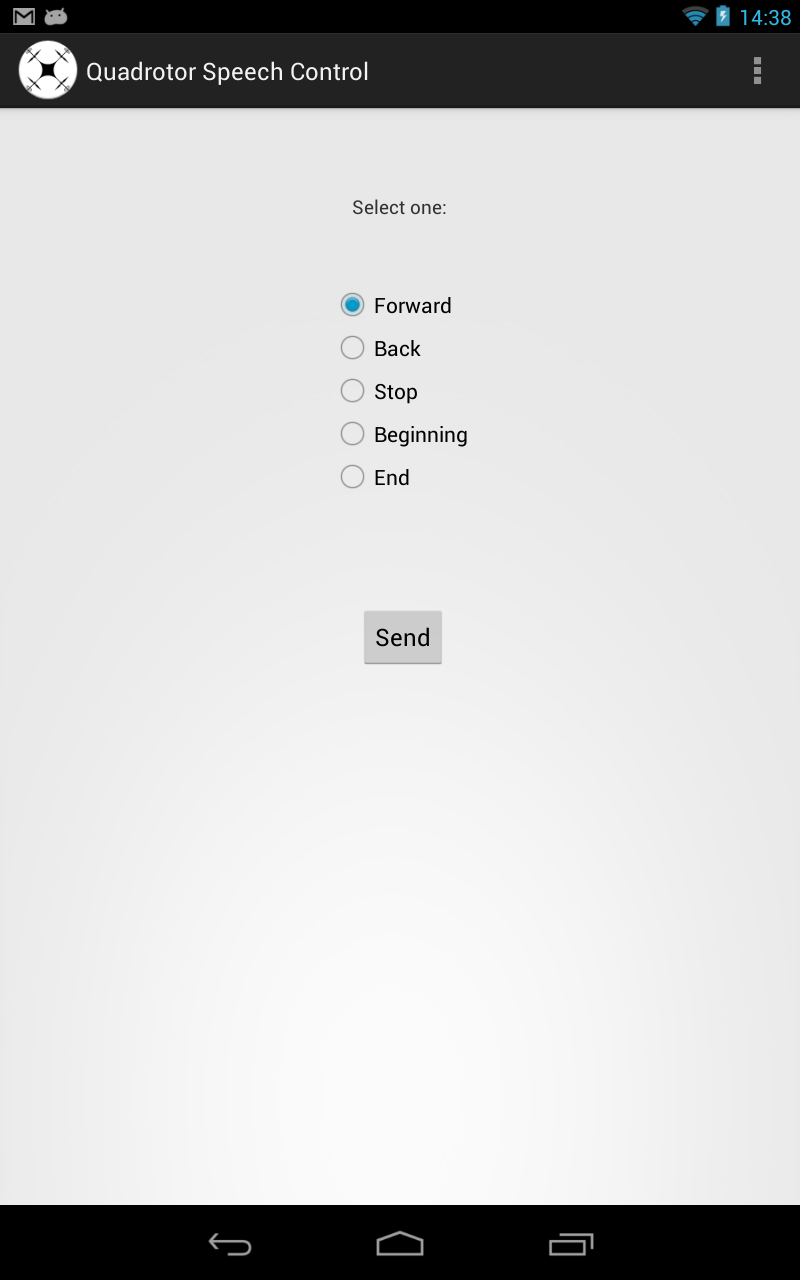
\includegraphics[scale=0.25]{figs/tablet2.png}
  \caption{Choice screen from the Android app}
  \label{fig:tablet_choice}
\end{figure}

\noindent Doing this allows us to avoid the pitfall of maximums with low probability and to be more robust during the following interactions. In fact the choice made by the user is not only used to send the proper command but also to label the interpretations of the speech recognizer and add them to the corpus.

\section{Simulation}

In order to test our approach composed a path using 8 markers and made the quadrotor follow it. The path is shown in Figure \ref{fig:path} where each marker is a square of 20cm side and the distance between each of them is 50cm; the quadrotor follows the path at a constant height of 2m. The size, the number and the distances of the tags, as well as the height of the quadrotor and the shape of the path, can be arbitrarily changed; the only restriction is that at least one tag need to be in the field of vision of the robot for all the duration of the simulation.

\begin{figure}[h!]
  \centering
    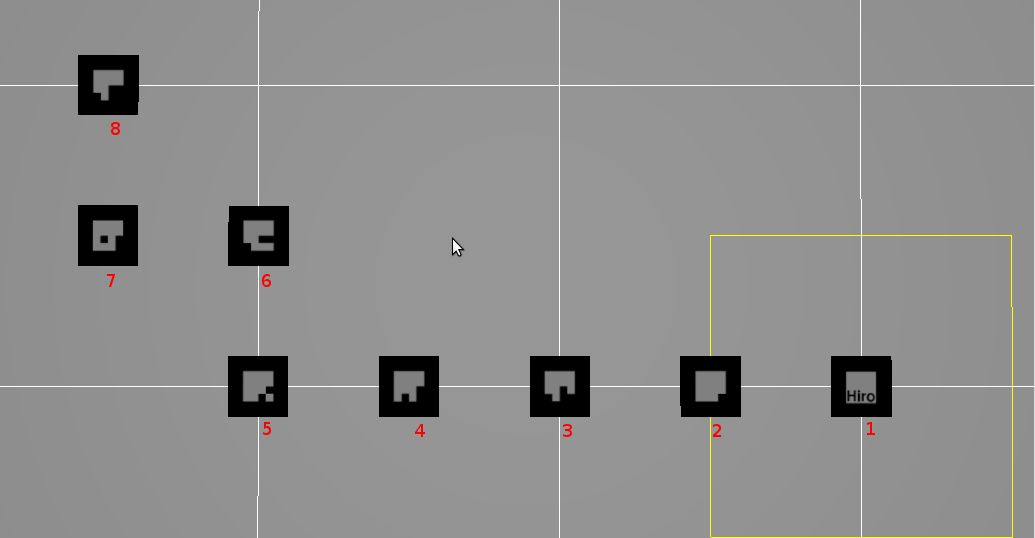
\includegraphics[scale=0.35]{figs/path.png}
  \caption{The path followed by the quadrotor during the simulations}
  \label{fig:path}
\end{figure}


In Figure \ref{fig:plot} we show the result of the first simulation. It can be seen that the estimate position along $X$ and $Y$ is very close to the real one, measured directly form the simulated environment. The plot for the position along the $Z$ axis appears at first more noisy but at a closer inspection we notice that the variation are in the order of $\pm$ 0.03 m that is very close to the maximum accuracy of ARTag ($\pm$ 0.02m).

\begin{figure}[h!]
  \centering
    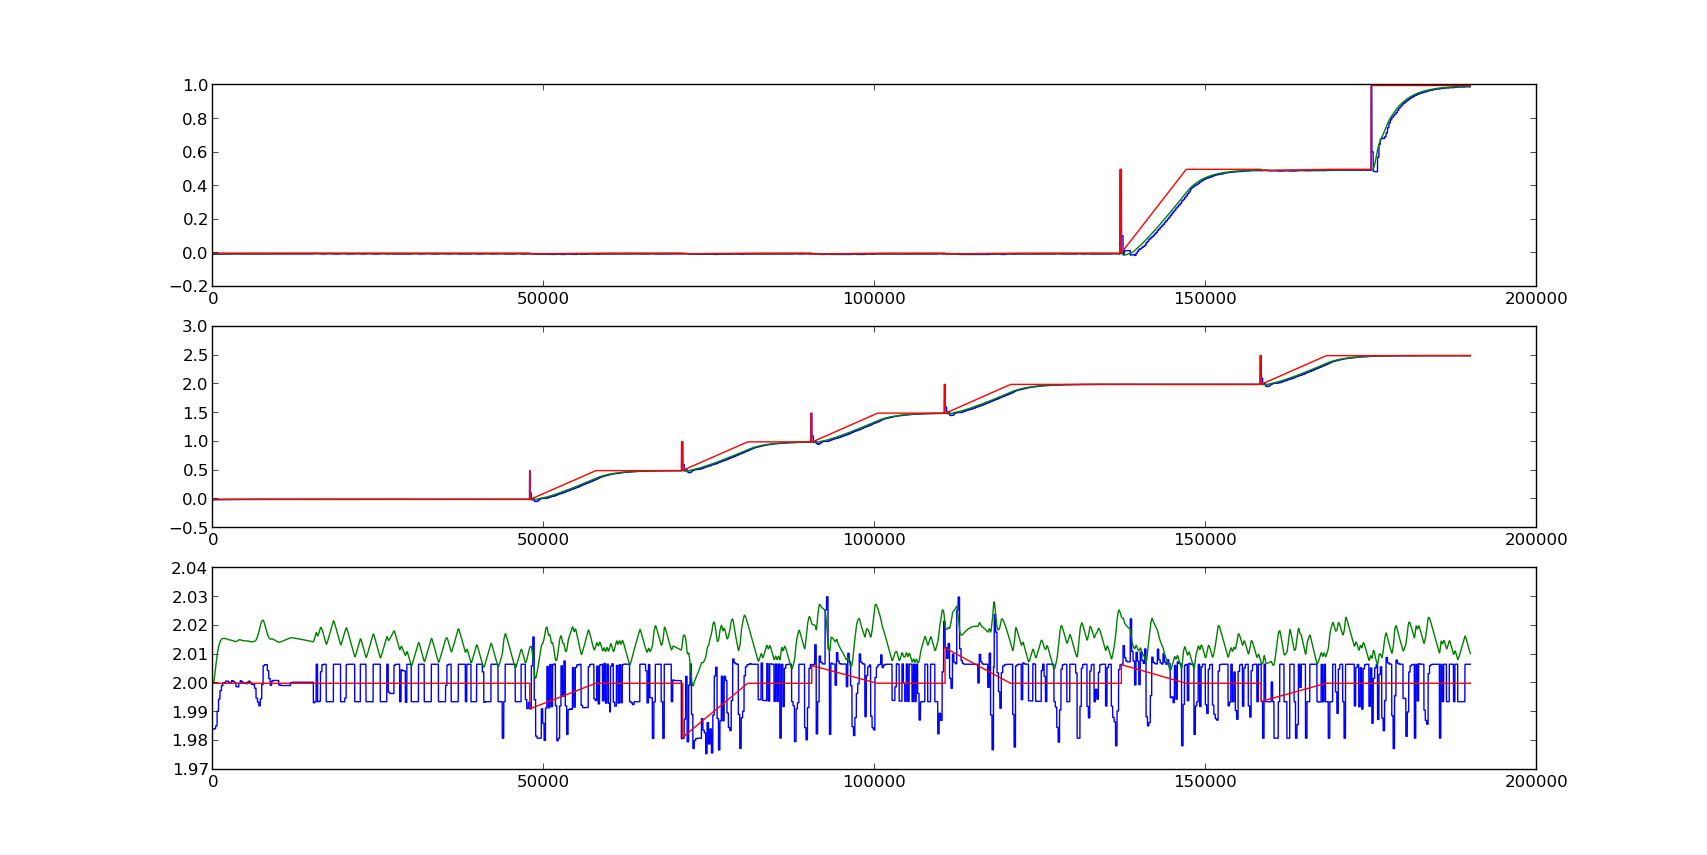
\includegraphics[scale=0.35]{figs/plot.png}
  \caption{Plot of desired, estimated and actual values for the position of the quadrotor}
  \label{fig:plot}
\end{figure}


To test the robustness of our approach and to better model real-environment conditions we ran a second simulation where we artificially introduced some noise. In particular the noise was added in two different ways, first we added both a Gaussian and a RGB noise on the image of the camera, Figure \ref{fig:artag} shows the difference of the perceived marker before and after the noise was added.

 \begin{figure}[!h]
 \centering
 \subfigure[ARTag with no noise]
   {
\includegraphics[width=4cm]{figs/artag.png}}
 \hspace{5mm}
 \subfigure[ARTag with Gaussian and RGB noise]
   {
\includegraphics[width=4cm]{figs/artag_noise.png}}
 \caption{Difference between tag wit and without noise}
 \label{fig:artag}
 \end{figure}
 

\noindent The second type of noise was added directly on the estimate of the position of ARTAg by adding to it an error computed according to a Gaussian distribution (INSERIRE PARAMETRI). In Figure \ref{fig:plot_noise} we show the result of this second simulation.

\begin{figure}[h!]
  \centering
    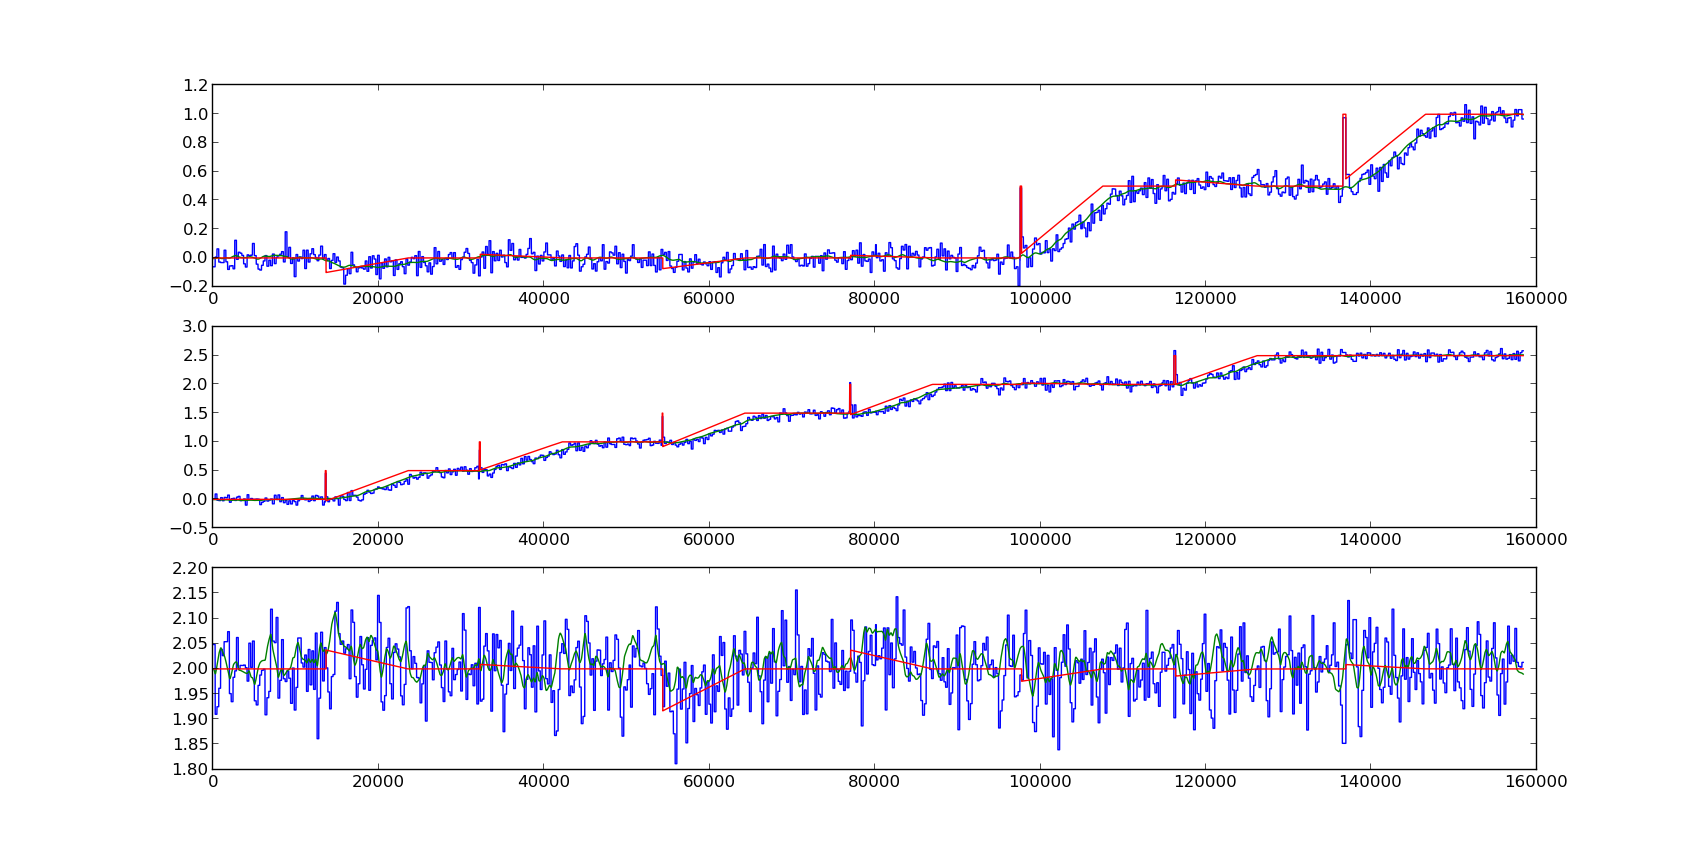
\includegraphics[scale=0.35]{figs/plot_noise.png}
  \caption{Plot of desired, estimated and actual values for the position of the quadrotor when noise was added}
  \label{fig:plot_noise}
\end{figure}


As can be seen even though some strong disturbance was introduced the estimate position is still close to the real one and the quadrotor is able to follow the path as planned. For this reason we believe that our approach could be applied not only in a simulation but to a real robot as well.

\appendix
\section{Installation}

Requisiti
procedure di installazione


\bibliography{biblio}
\bibliographystyle{plain}


\end{document}
